% Reconstructed from slides for Avanced Text Analysis MethodsNET Summer School.
% All text, equations, tables and diagrams are editable Beamer content.
% The resource-book collages on slides 9-10 are extracted images from the PDF.
\documentclass[11pt,aspectratio=43]{beamer}
\usepackage{amsmath,amssymb,booktabs,array,graphicx}
\usepackage{tikz}
\usetikzlibrary{arrows.meta,positioning,calc}
\usepackage{hyperref}

\setbeamertemplate{navigation symbols}{}
\setbeamercolor{structure}{fg=blue!55!black}
\setbeamercolor{frametitle}{fg=blue!55!black}
\setbeamercolor{itemize item}{fg=gray}
\setbeamercolor{itemize subitem}{fg=gray}
\setbeamercolor{author in head/foot}{fg=black,bg=white}
\setbeamercolor{title in head/foot}{fg=black,bg=white}
\setbeamercolor{date in head/foot}{fg=black,bg=white}
\setbeamercolor{johnbox}{fg=black,bg=blue!10}
\setbeamercolor{marybox}{fg=black,bg=green!12}
\setbeamertemplate{footline}{%
  \leavevmode\hbox{%
  \begin{beamercolorbox}[wd=.33\paperwidth,ht=2.5ex,dp=1ex,leftskip=1em]{author in head/foot}\scriptsize Tolochko \& Lebernegg \end{beamercolorbox}%
  \begin{beamercolorbox}[wd=.34\paperwidth,ht=2.5ex,dp=1ex,center]{title in head/foot}\scriptsize Advanced Text Analysis\end{beamercolorbox}%
  \begin{beamercolorbox}[wd=.33\paperwidth,ht=2.5ex,dp=1ex,rightskip=1em plus1fil]{date in head/foot}\hfill\scriptsize\insertframenumber/\inserttotalframenumber\end{beamercolorbox}}%
}
\setbeamertemplate{itemize items}[ball]
\setbeamersize{text margin left=1em,text margin right=1em}
\newcommand{\term}[1]{\texttt{#1}}
\newcommand{\prompt}[1]{\vspace{0.5em}\par\textcolor{blue!55!black}{\textbf{Discuss:}}~#1\par}
\newcommand{\source}[1]{\vfill{\scriptsize\textcolor{gray}{Source: #1}\par}}

\title{Advanced Quantitative Text Analysis}
\subtitle{Day 1: From Text to Measurement}
\author{Petro Tolochko, Noëlle Lebernegg}
\date{}

\begin{document}

% 1
\begin{frame}
  \titlepage
\end{frame}

% 2
\begin{frame}{Course Overview}
\begin{enumerate}
\item \textbf{Day 1:} Text representation, preprocessing, feature engineering
\item \textbf{Day 2:} Dictionaries, supervised, and unsupervised classification
\item \textbf{Day 3:} Embeddings, transformers, LLMs
\item \textbf{Day 4:} Multilingual analysis, evaluation, research design, project talk
\end{enumerate}
\end{frame}

% 6
\begin{frame}{Objectives}
\begin{itemize}
\item Understand major approaches to automated text analysis
\item Learn how text is transformed into data
\item Identify practical challenges in real text-analysis projects
\item Critically evaluate representation and modeling choices
\item Connect methods to your own research questions
\end{itemize}
\end{frame}

% 3
\begin{frame}{Course Structure}
\begin{itemize}
\item Theoretical input
\item Practical sessions
\item Discussion of participants' own projects
\item Focus on method choice, validation, and research design
\end{itemize}
\end{frame}

% 4
\begin{frame}{Introduction}
Petro Tolochko
\begin{itemize}
\item Post-Doc, Computational Communication Science Lab, University of Vienna
\item Research focus: text complexity, social networks, statistical modeling
\item \texttt{petro.tolochko@univie.ac.at}
\end{itemize}
\vspace{1em}
Noelle Lebernegg
\begin{itemize}
\item Post-Doc, Strategic Communication Science Group, Wageningen Univeristy
\item Research focus: text as data, data mining, statistical modeling
\item \texttt{noelle.lebernegg@wur.nl}
\end{itemize}
\end{frame}

% 5
\begin{frame}{Introduction: Participants}
\begin{itemize}
\item Name?
\item Disciplinary background?
\item Experience with text analysis?
\item Programming experience?
\item Expectations / wishes for the workshop?
\end{itemize}
\end{frame}

% 3
\begin{frame}{Course Assessment}
\begin{itemize}
\item In-class participation (20\%)\\
\item Final paper: application of one or several automated text analysis methods on a topic related to a topic of interest (e.g., related to your PhD thesis) (80\%)
\begin{itemize}
\item Content: short motivation, analysis (incl. commented code), description and interpretation of results (about 10 pages)
\item Format: Jupyter notebook (.ipynb) or R Markdown (.Rmd)
\item Deadline: 31. January, 2026
\item Project Talk: Day 4, afternoon
\end{itemize}
\end{itemize}
\end{frame}

% 7
\begin{frame}{Course Resources}
Course repository:
\begin{itemize}
\item \url{https://github.com/PeterTolochko/MethodsNET_Summer_School}
\item Code, datasets, notebooks, and exercises will be organized there.
\end{itemize}
\end{frame}

% 7
\begin{frame}{Some Python Resources}
\begin{itemize}
\item Van der Plas, J. (2026). Python Data Science Handbook: Essential Tools \url{https://github.com/jakevdp/PythonDataScienceHandbook}
\end{itemize}
\end{frame}


% 7
\begin{frame}{Some R Resources}
\begin{itemize}
\item R for Data Science: \url{https://r4ds.had.co.nz/}
\item Tidy Modeling with R: \url{https://www.tmwr.org/}
\item Big Book of R. Database of R resources. \url{https://www.bigbookofr.com}
\end{itemize}
\end{frame}


% 7
\begin{frame}{R and Python Ressources for Text Analysis}
\begin{itemize}
\item Atteveldt, W., Trilling, D., \& Arcila, C. (2021). Computational Analysis of Communication. Wiley-Blackwell. \url{http://cssbook.net}
\item Hugging Face. NLP Course. \url{https://huggingface.co/learn/nlp-course/chapter0/1}
\end{itemize}
\end{frame}

\begin{frame}{Books for the course}
\textbf{Grimmer, Roberts \& Stewart (2022)}\\
\href{https://politicalscience.stanford.edu/publications/text-data-new-framework-machine-learning-and-social-sciences}{\textcolor{blue!50!black}{\textit{Text as Data}}}\\
Research design and measurement with text.\\
\vspace{5mm}
\textbf{Jurafsky \& Martin}\\
\href{https://web.stanford.edu/~jurafsky/slp3/}{\textcolor{blue!50!black}{\textit{Speech and Language Processing}}}\\
NLP methods and language models. Free third-edition draft.
\vspace{5mm}

\textbf{James et al.\ (2023)}\\
\href{https://www.statlearning.com/}{\textcolor{blue!50!black}{\textit{An Introduction to Statistical Learning}}}\\
Python edition. Model fitting and evaluation. Free PDF.
\note{These are recommended references. Briefly explain which book helps with which part of the course. Grimmer, Justin, Margaret E. Roberts, and Brandon M. Stewart (2022), Text as Data: A New Framework for Machine Learning and the Social Sciences, Princeton University Press. Jurafsky, Dan, and James H. Martin, Speech and Language Processing, third-edition online draft, release dated August 19, 2026 when checked. James, Gareth, Daniela Witten, Trevor Hastie, Robert Tibshirani, and Jonathan Taylor (2023), An Introduction to Statistical Learning: with Applications in Python, Springer. Titles link to the official book or author-institution pages. Verified September 14, 2026: \url{https://politicalscience.stanford.edu/publications/text-data-new-framework-machine-learning-and-social-sciences}, \url{https://web.stanford.edu/~jurafsky/slp3/}, \url{https://www.statlearning.com/}.}
\end{frame}

\begin{frame}{Further reading and practical references}
\textbf{Manning, Raghavan \& Sch\"utze (2008)}\\
\href{https://nlp.stanford.edu/IR-book/}{\textcolor{blue!50!black}{\textit{Introduction to Information Retrieval}}}\\
Word counts, TF-IDF, and vector similarity. Free online.
\vspace{5mm}

\textbf{Cosma Rohilla Shalizi}\\
\href{https://www.stat.cmu.edu/~cshalizi/ADAfaEPoV/}{\textcolor{blue!50!black}{\textit{Advanced Data Analysis}}}\\
\textit{from an Elementary Point of View}\\
Statistical reasoning and model evaluation. Free draft, R examples.

\end{frame}

% 8
\begin{frame}{Today}
\begin{itemize}
\item Text as data, text as measurement
\item Document-term matrices and bag-of-words
\item Preprocessing as an analytical choice
\item TF-IDF and feature weighting
\item Similarity, distance, and comparing texts
\item Practical: how representation changes results
\end{itemize}
\end{frame}


% 12
\begin{frame}{Why Analyse Texts?}
\begin{itemize}
\item Vast quantities of textual data are available
\item Texts carry meaning
\item Texts capture social, political, and cultural behaviour
\item Texts can help us study phenomena that are otherwise difficult to observe
\end{itemize}
\end{frame}

% 13
\begin{frame}{What Do We Measure Through Text?}
\begin{itemize}
\item We usually do not analyse text "for its own sake"
\item We use text to measure latent or difficult-to-observe concepts:
  \begin{itemize}
  \item attention \quad sentiment \quad framing \quad ideology
  \item complexity \quad toxicity \quad uncertainty \quad polarization
  \end{itemize}
\item The representation determines what the model can measure
\end{itemize}
\end{frame}

% 14
\begin{frame}{The Text Analysis Pipeline}
\centering
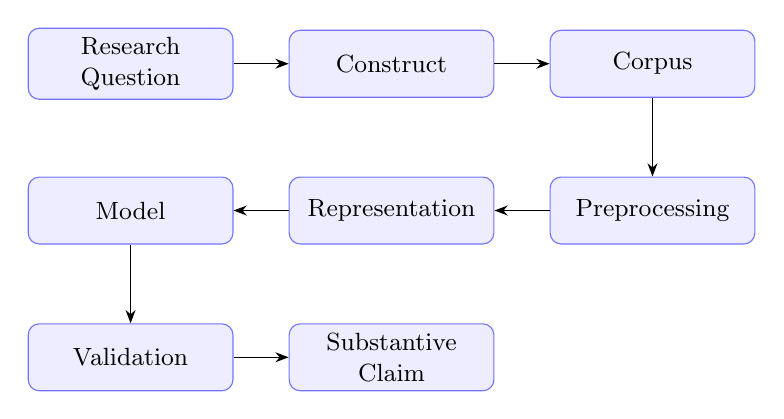
\begin{tikzpicture}[>=Stealth,box/.style={draw=blue!55,fill=blue!7,rounded corners,minimum width=2.6cm,minimum height=.85cm,align=center,font=\small},node distance=1.0cm and .7cm]
\node[box] (rq) {Research\\Question};
\node[box,right=of rq] (construct) {Construct};
\node[box,right=of construct] (corpus) {Corpus};
\node[box,below=of corpus] (pre) {Preprocessing};
\node[box,left=of pre] (repr) {Representation};
\node[box,left=of repr] (model) {Model};
\node[box,below=of model] (valid) {Validation};
\node[box,right=of valid] (claim) {Substantive\\Claim};
\draw[->] (rq)--(construct); \draw[->] (construct)--(corpus);
\draw[->] (corpus)--(pre); \draw[->] (pre)--(repr);
\draw[->] (repr)--(model); \draw[->] (model)--(valid);
\draw[->] (valid)--(claim);
\end{tikzpicture}
\end{frame}


% Research examples and text as measurement.
\begin{frame}{Research questions and text}
Texts record what people choose to say or write.
\vspace{5mm}
\begin{itemize}
\item Speeches can reveal political attention
\item News articles can reveal how an issue is framed
\item Open survey responses can reveal concerns that fixed questions miss
\end{itemize}
\note{These are possible research uses. The following papers illustrate how researchers turn texts into evidence for different questions. After these examples, introduce the jobs question that we will work through together.}
\end{frame}


\begin{frame}{Censorship in digitized books}
Can changes in name frequency reveal censorship?
\vspace{5mm}
\begin{columns}[c,onlytextwidth]
\column{0.57\textwidth}
% Panel A only. Place the axis title outside the crop to exclude panel C.
{\centering
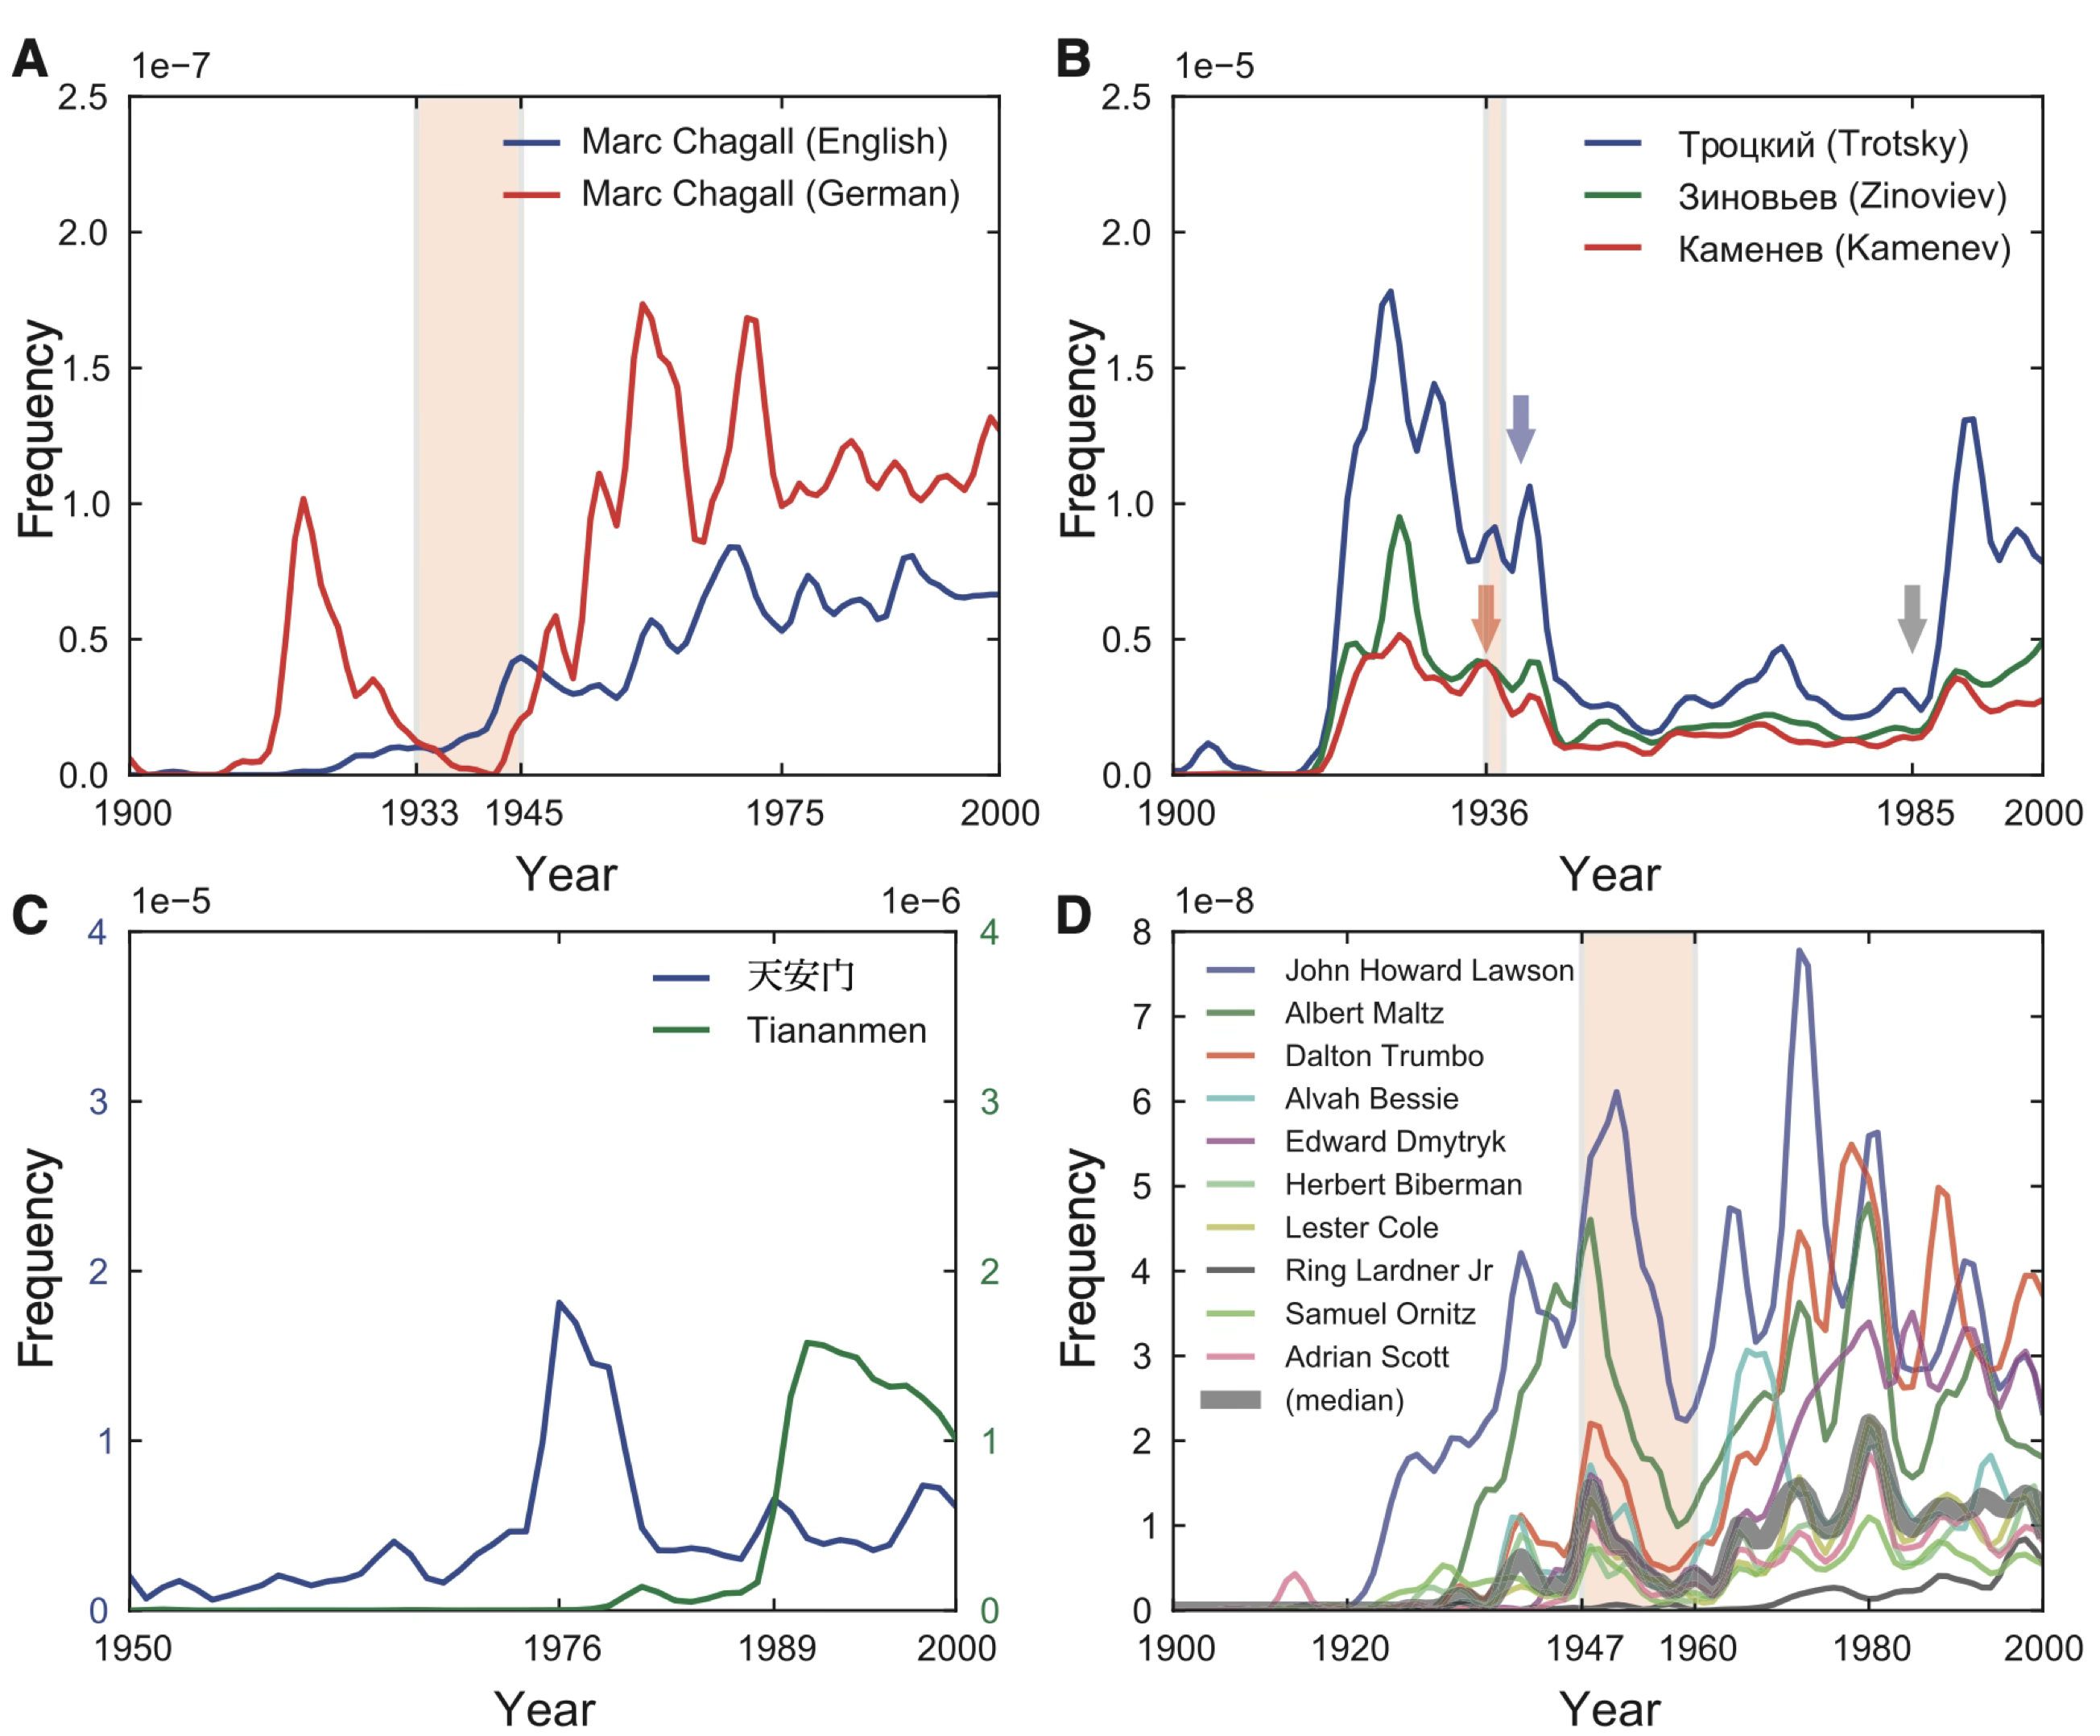
\includegraphics[width=0.94\linewidth,trim=0bp 548bp 655bp 0bp,clip]{figures/michel2011_figure4.png}\par
\vspace{-0.1em}{\small Year}\par}
\column{0.40\textwidth}
\small
\textbf{Texts}\\
English and German books
\vspace{5mm}
\textbf{Measure}\\
Frequency of ``Marc Chagall'' by year
\vspace{5mm}
\textbf{Pattern}\\
German mentions nearly disappear during Nazi rule
\end{columns}
\prompt{What else could make a name disappear from books?}
\source{\href{https://doi.org/10.1126/science.1199644}{Michel et al.\ (2011), \textit{Science}, Figure 4A.}}
\note{Spend about two minutes. Source: Michel et al. (2011), Quantitative Analysis of Culture Using Millions of Digitized Books, Science 331:176--182, doi:10.1126/science.1199644. The authors interpret this language contrast as evidence of censorship. Ask how changes in corpus composition, spelling, or OCR quality could affect the inference. The figure shows normalized frequencies, not raw counts. We reuse the figure from the earlier course materials and crop to panel A without changing the data. Source text checked at \url{https://pmc.ncbi.nlm.nih.gov/articles/PMC3279742/}.}
\end{frame}

\begin{frame}{Policy adoption and newspaper framing}
Do policies adopted elsewhere predict how newspapers discuss smoking restrictions?
\vspace{5mm}
\textbf{Texts:} over 52,000 newspaper paragraphs\\
49 US states, 1996--2013
\vspace{5mm}
\textbf{Result from the topic-model analysis}
\begin{center}
\small
\begin{tabular}{p{0.43\linewidth}p{0.46\linewidth}}
\toprule
\textbf{Framing of the policy} & \textbf{Earlier adoptions elsewhere} \\
\midrule
Practical consequences & Predictive relationship \\[0.5em]
Normative justifications & No predictive relationship \\
\bottomrule
\end{tabular}
\end{center}
\source{\href{https://doi.org/10.1111/ajps.12521}{Gilardi, Shipan \& W\"uest (2021), \textit{AJPS}.}}
\note{Spend about three minutes. Source: Gilardi, Shipan, and W\"uest (2021), Policy Diffusion: The Issue-Definition Stage, American Journal of Political Science 65:21--35, doi:10.1111/ajps.12521. Explain normative justifications as arguments about why a restriction is right or justified. The table summarizes the abstract and reports no effect sizes or causal identification claim. Introduce a topic as a pattern of words that researchers interpret, then return to validation by reading paragraphs. Possible student answers: read the paragraph and identify its main argument; define practical consequences as claims about outcomes (restaurant revenue, enforcement costs) and normative justifications as claims about rights, fairness, or what ought to be done; use words as clues but check them in context; let two readers classify the same paragraphs and discuss disagreements. A paragraph may contain both frames. Illustrative examples, not quotations from the paper: restrictions could reduce restaurant revenue (consequences); workers have a right to clean air (normative justification). Defer model details. Source checked against the journal abstract and the original course slide.}
\end{frame}

\begin{frame}{Is online communication an echo chamber?}
\textbf{Barber\'a et al.\ (2015):} does information travel across ideological boundaries?
\vspace{5mm}
\small
Nearly 150 million tweets on 12 political and nonpolitical issues; estimated ideology for 3.8 million users.
\begin{center}
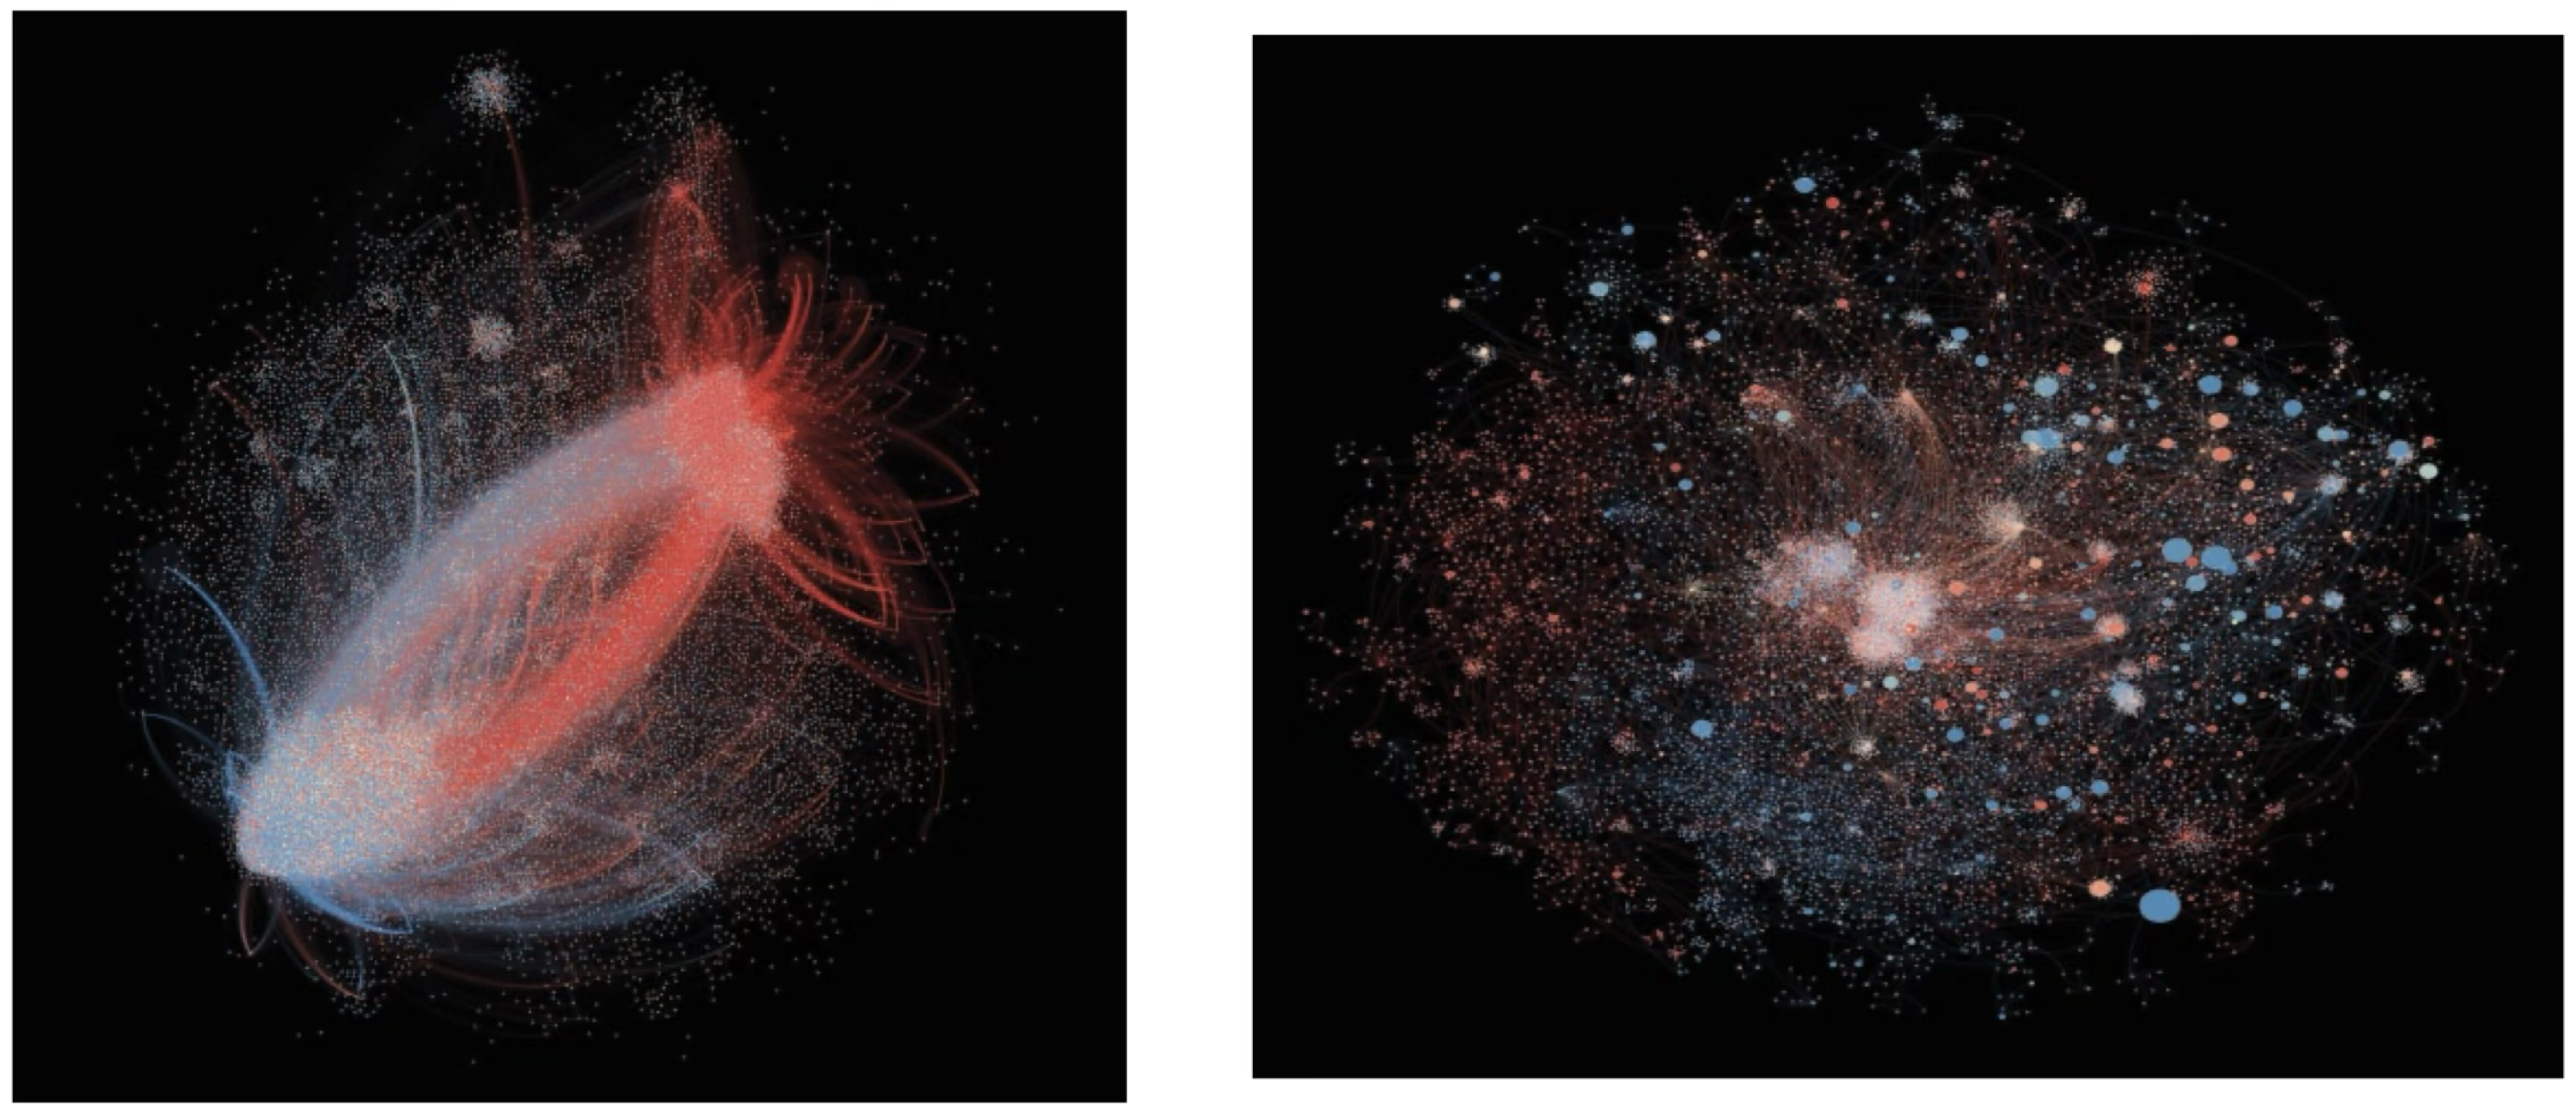
\includegraphics[width=0.80\linewidth]{figures/barbera2015_networks.png}
\end{center}
Political issues showed more exchange among ideologically similar users; many nonpolitical events did not.
\source{\href{https://doi.org/10.1177/0956797615594620}{Barber\'a et al.\ (2015), \textit{Tweeting From Left to Right}, Psychological Science.}}
\note{Reuse the network comparison shown in CEU 2025. Ask students to compare separation and mixing in the two networks, without treating the drawing's coordinates as word-count dimensions. The study combines communication content with network information: ideology is estimated from network behavior, not a simple count of liberal and conservative words. Political cases include the 2012 presidential election and 2013 government shutdown; nonpolitical cases include the 2013 Boston Marathon bombing and 2014 Super Bowl. These are examples from the abstract, not labels assigned to the two image panels. Authors: Pablo Barber\'a, John T. Jost, Jonathan Nagler, Joshua A. Tucker, and Richard Bonneau. Psychological Science 26(10):1531--1542. The research lesson is that the answer depends on which conversations we study.}
\end{frame}

\begin{frame}{First measurment?}
How much attention do US presidents give to jobs in their State of the Union speeches?
\vspace{5mm}
We will start by reading passages, then build and check a simple word-count indicator.
\note{Transition from the published research examples to our shared exercise. Ask what kind of evidence would answer the jobs question. Separate attention expressed in a speech from a politician's private priorities, later policy, or public opinion. The next slide begins with two passages from the teaching sample.}
\end{frame}

\begin{frame}{Jobs in presidential speeches}
\textbf{Barack Obama, 2010}
\begin{quote}
``That is why jobs must be our number-one focus in 2010, and that's why I'm calling for a new jobs bill tonight.''
\end{quote}
\vspace{5mm}
\textbf{Donald Trump, 2020}
\begin{quote}
``Jobs are booming, incomes are soaring, poverty is plummeting, crime is falling, confidence is surging, and our country is thriving and highly respected again.''
\end{quote}
\prompt{Do these passages express the same thing about jobs?}
\note{Allow students to distinguish attention, tone, and a policy demand. Both passages mention jobs. Their evaluative content and rhetorical purpose differ. A good answer: Obama presents employment as a priority requiring action and calls for a jobs bill; Trump presents jobs as evidence that the economy is doing well. One passage makes a policy demand, while the other makes a positive assessment. Counting job/jobs can indicate attention to employment, but does not distinguish those meanings. Do not infer a negative sentiment label for Obama merely from his call for action. The quotations reproduce the local teaching corpus and do not establish the truth of the speakers' economic claims.}
\end{frame}

\begin{frame}{A concept and a first indicator}
\textbf{Concept:} attention to employment in a speech
\vspace{5mm}
\textbf{First indicator:} occurrences of \texttt{job} or \texttt{jobs}
\[
\text{mentions per 1,000 tokens}
=\frac{\text{count of job + jobs}}{\text{number of tokens}}\times 1{,}000
\]
\begin{itemize}
\item A longer speech has more opportunities to mention a word
\item A rate makes speeches of different lengths easier to compare
\end{itemize}
\prompt{Which discussions of employment would this count miss?}
\note{Possible answers: unemployment, hiring, wages, layoffs, work, occupations. This rate is a deliberately simple indicator. Repetition, ambiguity, and different rhetorical contexts all affect its interpretation. A larger dictionary would introduce further choices and still require validation.}
\end{frame}

\begin{frame}{Checking the indicator against the text}
\textbf{Another use of ``jobs'' in Obama's 2010 speech}
\begin{quote}
``That's why we've excluded lobbyists from policymaking jobs or seats on Federal boards and commissions.''
\end{quote}
\vspace{5mm}
\begin{itemize}
\item Read passages that the indicator counts
\item Look for relevant passages that it misses
\item Decide what counts as attention to employment
\end{itemize}
\prompt{Would you include this passage? Why?}
\note{There is no automatic answer: it depends on the definition of the construct. The point is to specify a coding rule and assess the indicator against it. This introduces validation without teaching classification metrics yet.}
\end{frame}


\begin{frame}{Exercise: First text analysis project idea}
\begin{itemize}
\item Form groups (of two to three people)
\item Discuss initial text analysis project ideas
\vspace{1em}
\item[$\rightarrow$] You can talk about project ideas that you already have or about areas in your discipline where large text quantities play a role  
\end{itemize}
\end{frame}


\begin{frame}[plain]
  \centering
  \vfill
  {\usebeamercolor[fg]{structure}\LARGE\bfseries
   From Text to Structure\par}
  \vfill
\end{frame}

% 16
\begin{frame}{What is Text?}
\begin{itemize}
\item Data
\item Unstructured
\item Highly multidimensional
\item Difficult to work with if you are not human
\end{itemize}
\end{frame}

% 15
\begin{frame}{The Basic Problem}
\begin{itemize}
\item Text is meaningful to humans
\item But computers do not directly "understand" text
\item We need to transform text into structured representations
\end{itemize}
\end{frame}

% 17
\begin{frame}{From Text to Structure}
\begin{itemize}
\item We need to structure text before analysis
\item We need representations that computers can process
\item We also need representations that remain meaningful to us (and our research questions)
\item Different research questions $\rightarrow$ different representations
\end{itemize}
\end{frame}

% 18
\begin{frame}{Unit of Analysis}
\scriptsize
\begin{tabular}{p{.49\textwidth}p{.44\textwidth}}
\toprule
\textbf{Research question} & \textbf{Possible unit}\\ \midrule
Does newspaper coverage become more negative? & article / paragraph / sentence\\
Do parties use simpler language? & speech / manifesto / paragraph\\
Are social-media posts toxic? & post / comment\\
What topics dominate climate discourse? & article / document / sentence\\
\bottomrule
\end{tabular}
\vspace{1em}
\begin{itemize}\item Unit choice determines what the model can see\end{itemize}
\end{frame}

% 19
\begin{frame}{Document-Term Matrix}
\[
X=N\times K
\]
\begin{itemize}
\item $N$ = number of documents
\item $K$ = number of terms/features
\item $X$ = structured representation of the corpus
\end{itemize}
\end{frame}

% 20
\begin{frame}{Document-Term Matrix}
\[
X=\begin{bmatrix}
1&1&1&0&0&0\\
1&1&0&1&0&0\\
0&0&1&0&1&1
\end{bmatrix}
\]
\[
N=3,\qquad K=6
\]
\end{frame}

% 21
\begin{frame}{Example Corpus}
\begin{itemize}
\item Doc 1: "John loves ice-cream"
\item Doc 2: "John loves oranges"
\item Doc 3: "Mary hates ice-cream"
\end{itemize}
\[
N=?,\qquad K=?,\qquad X=?
\]
\end{frame}

% 22
\begin{frame}{Document-Term Matrix with Vocabulary}
\centering
\scriptsize
\begin{tabular}{c|rrrrrr}
 & John & loves & ice-cream & oranges & Mary & hates\\ \hline
$D_1$&1&1&1&0&0&0\\
$D_2$&1&1&0&1&0&0\\
$D_3$&0&0&1&0&1&1
\end{tabular}
\vspace{1.5em}
\[
N=3,\qquad K=6,\qquad X\in\mathbb{R}^{3\times6}
\]
\end{frame}

% 23
\begin{frame}{Types \& Tokens}
\begin{itemize}
\item \textbf{Tokens:} all word occurrences
\item \textbf{Types:} unique word forms
\end{itemize}
\vspace{1em}
Example corpus:
\begin{itemize}
\item 9 tokens
\item 6 types
\end{itemize}
\end{frame}

% 24
\begin{frame}{Bag-of-Words Representation}
\begin{itemize}
\item Representation of text as a bag of words
\item Word order is ignored
\item Each document is represented as counts of words
\item Simple, powerful, and still widely used
\end{itemize}
\end{frame}

% 25
\begin{frame}{What Bag-of-Words Captures and Loses}
\begin{columns}[T]
\begin{column}{.48\textwidth}
\textbf{Captures}
\begin{itemize}
\item word frequency
\item topical emphasis
\item repeated lexical choices
\item broad document similarity
\end{itemize}
\end{column}
\begin{column}{.48\textwidth}
\textbf{Loses}
\begin{itemize}
\item word order
\item syntax
\item negation scope
\item irony and sarcasm
\item who did what to whom
\end{itemize}
\end{column}
\end{columns}
\end{frame}

% 26
\begin{frame}{Bag-of-Words Is an Abstraction}
\begin{itemize}
\item Bag-of-words is not "stupid"
\item It deliberately discards some information
\item It keeps information that is often useful:
  \begin{itemize}
  \item lexical choice
  \item frequency
  \item relative emphasis
  \item co-occurrence across documents
  \end{itemize}
\item Whether this abstraction is appropriate depends on the research question
\end{itemize}
\end{frame}

% 27
\begin{frame}{Sparse High-Dimensional Data}
\begin{itemize}
\item Most corpora have many unique terms
\item Most documents contain only a small fraction of all terms
\item Result: document-term matrices are usually sparse
\item This affects modeling, storage, computation, and interpretation
\end{itemize}
\end{frame}

\begin{frame}[plain]
  \centering
  \vfill
  {\usebeamercolor[fg]{structure}\LARGE\bfseries
   Word counts as a probability\par}
  \vfill
\end{frame}

% 28
\begin{frame}{Multinomial Model of Language}
\begin{itemize}
\item Text $\approx$ draw from a Multinomial distribution
\end{itemize}
\end{frame}

% 29
\begin{frame}{Binomial Distribution}
\[
P(X=k)=\binom{n}{k}p^k(1-p)^{n-k}
\]
\begin{itemize}
\item $n$ = number of trials
\item $k$ = number of successes
\item $p$ = success probability
\end{itemize}
\end{frame}

% 30
\begin{frame}{Multinomial Distribution}
\[
P(X_1=x_1,\ldots,X_k=x_k)=
\frac{n!}{x_1!x_2!\cdots x_k!}
p_1^{x_1}p_2^{x_2}\cdots p_k^{x_k}
\]
where: $n$ = text length,\quad $k$ = vocabulary size,\quad
$p_i$ = probability of word $i$
\end{frame}

% 31
\begin{frame}{Binomial vs. Multinomial}
\begin{itemize}
\item \textbf{Binomial:} one word (success/failure)
\[
P(X=k)=\binom{n}{k}p^k(1-p)^{n-k}
\]
\item \textbf{Multinomial:} multiple words/categories
\[
P(x_1,\ldots,x_k)=\frac{n!}{x_1!\cdots x_k!}\prod_{i=1}^k p_i^{x_i}
\]
\end{itemize}
\end{frame}

% 32
\begin{frame}{Example Texts}
\small
\begin{itemize}
\item Text 1 = banana banana banana banana chocolate
\item Text 2 = chocolate chocolate chocolate banana fudge
\item Text 3 = banana banana
\item Text 4 = ice-cream ice-cream fudge ice-cream banana chocolate
\item Text 5 = fudge fudge fudge chocolate
\item Text 6 = ice-cream chocolate ice-cream fudge fudge fudge
\end{itemize}
\end{frame}

% 33
\begin{frame}{Example Texts}
\scriptsize
\begin{beamercolorbox}[rounded=true,shadow=true,sep=.7ex,wd=\textwidth]{johnbox}
\textbf{John}\\
Text 1 = banana banana banana banana chocolate\\
Text 2 = chocolate chocolate chocolate banana fudge\\
Text 3 = banana banana
\end{beamercolorbox}
\vspace{.7em}
\begin{beamercolorbox}[rounded=true,shadow=true,sep=.7ex,wd=\textwidth]{marybox}
\textbf{Mary}\\
Text 4 = ice-cream ice-cream fudge ice-cream banana chocolate\\
Text 5 = fudge fudge fudge chocolate\\
Text 6 = ice-cream chocolate ice-cream fudge fudge fudge
\end{beamercolorbox}
\end{frame}

% 34
\begin{frame}{Document-Term Matrix}
\centering
\small
\begin{tabular}{l|rrrr}
 & banana & chocolate & fudge & icecream\\ \hline
Doc 1&4&1&0&0\\
Doc 2&1&3&1&0\\
Doc 3&2&0&0&0\\
Doc 4&1&1&1&3\\
Doc 5&0&1&3&0\\
Doc 6&0&1&3&2
\end{tabular}
\end{frame}

% 35
\begin{frame}{Document-Term Matrix}
\centering
\small
\begin{tabular}{l|rrrr}
 & banana & chocolate & fudge & icecream\\ \hline
John Rates&7&4&1&0\\
Mary Rates&1&3&7&5
\end{tabular}
\end{frame}

% 36
\begin{frame}{Language Models}
\begin{block}{John Language Model}
John Rates \qquad 7 \qquad 4 \qquad 1 \qquad 0
\end{block}
\vspace{1em}
\begin{exampleblock}{Mary Language Model}
Mary Rates \qquad 1 \qquad 3 \qquad 7 \qquad 5
\end{exampleblock}
\end{frame}

% 37
\begin{frame}{Language Models}
\begin{block}{John Language Model}
John Rates \qquad $\frac{7}{12}$ \qquad $\frac{4}{12}$ \qquad $\frac{1}{12}$ \qquad $\frac{0}{12}$
\end{block}
\vspace{1em}
\begin{exampleblock}{Mary Language Model}
Mary Rates \qquad $\frac{1}{16}$ \qquad $\frac{3}{16}$ \qquad $\frac{7}{16}$ \qquad $\frac{5}{16}$
\end{exampleblock}
\end{frame}

% 38
\begin{frame}{New Texts}
\begin{itemize}
\item \term{new\_text\_1} = ice-cream fudge fudge
\item \term{new\_text\_2} = chocolate chocolate banana banana
\end{itemize}
\vspace{1em}
Question: Probability they were generated by John or Mary?
\end{frame}

% 39
\begin{frame}{New Texts Document-Term Matrix}
\centering
\small
\begin{tabular}{l|rrrr}
 & banana & chocolate & fudge & icecream\\ \hline
New Text 1 Rates&0&0&2&1\\
New Text 2 Rates&2&2&0&0
\end{tabular}
\end{frame}

% 40
\begin{frame}{Probability Spoken by John}
\begin{itemize}
\item \term{new\_text\_1} = "ice-cream fudge fudge"
\end{itemize}
\[
\begin{aligned}
\Pr(b=0,ch=0,f=2,i=1)
&=\frac{3!}{0!0!2!1!}\\
&\quad\times(0.583)^0(0.333)^0(0.08)^2(0)^1\\
&=0
\end{aligned}
\]
\end{frame}

% 41
\begin{frame}{Probability Spoken by John}
\begin{itemize}
\item \term{new\_text\_2} = "chocolate chocolate banana banana"
\end{itemize}
\[
\begin{aligned}
\Pr(b=2,ch=2,f=0,i=0)
&=\frac{4!}{2!2!0!0!}
(0.583)^2(0.333)^2(0.08)^0(0)^0\\
&=6(0.583)^2(0.333)^2\\
&\approx0.23
\end{aligned}
\]
\end{frame}

% 42
\begin{frame}{Probability spoken by Mary}
\begin{itemize}
\item \term{new\_text\_1} (Mary): $\Pr=0.18$
\item \term{new\_text\_2} (Mary): $\Pr=0.0008$
\end{itemize}
\end{frame}

\begin{frame}[plain]
  \centering
  \vfill
  {\usebeamercolor[fg]{structure}\LARGE\bfseries
   Documents as vectors\par}
  \vfill
\end{frame}

% 43
\begin{frame}{Vector Space Model}
\begin{itemize}
\item Represent texts as vectors in multidimensional space
\item Each dimension corresponds to a feature
\item In a document-term matrix, features are usually words or phrases
\item Once texts are vectors, we can compare them geometrically
\end{itemize}
\end{frame}

% 44
\begin{frame}{Multidimensional Spaces}
Multidimensional?
\begin{itemize}
\item 2D: position on a map\\
$X$ = longitude, $Y$ = latitude
\item 3D: position in the real world\\
$X$ = longitude, $Y$ = latitude, $Z$ = height
\item 4D:\\
$X$ = longitude, $Y$ = latitude, $Z$ = height, $T$ = time
\end{itemize}
\end{frame}

% 45
\begin{frame}{Multidimensional Spaces}
\begin{itemize}
\item The number of dimensions is the number of features needed to describe an object
\item In geography: coordinates describe location
\item In text analysis: words/features describe the position of a document in linguistic space
\end{itemize}
\end{frame}

% 46
\begin{frame}{Two-Dimensional Space}
Vocabulary = \{"banana", "chocolate"\}
\begin{itemize}
\item Text 1 = "chocolate chocolate chocolate banana"
\item Text 2 = "banana banana banana banana chocolate"
\item Text 3 = "banana banana"
\end{itemize}
\end{frame}

% 47
\begin{frame}{Two-Dimensional Space}
Vocabulary = \{"banana", "chocolate"\}
\begin{itemize}
\item Text 1 = "chocolate chocolate chocolate banana" $\Rightarrow(1,3)$
\item Text 2 = "banana banana banana banana chocolate" $\Rightarrow(4,1)$
\item Text 3 = "banana banana" $\Rightarrow(2,0)$
\end{itemize}
\end{frame}

% 48
\begin{frame}{Two-Dimensional Vector Space}
\centering
\begin{tikzpicture}[scale=.95,>=Stealth]
\draw[->] (0,0)--(5.2,0) node[right]{banana};
\draw[->] (0,0)--(0,4.2) node[above]{chocolate};
\fill[blue] (1,3) circle (2.4pt) node[above left]{Text 1 (1,3)};
\fill[red] (4,1) circle (2.4pt) node[right]{Text 2 (4,1)};
\fill[green!60!black] (2,0) circle (2.4pt) node[below]{Text 3 (2,0)};
\end{tikzpicture}
\end{frame}

% 49
\begin{frame}{Two-Dimensional Vector Space}
\centering
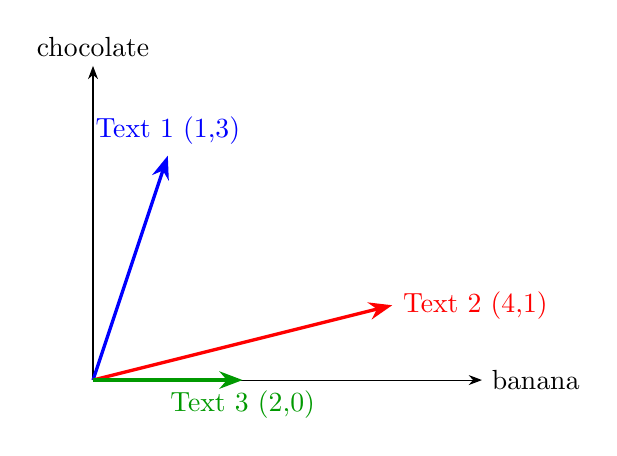
\begin{tikzpicture}[scale=.95,>=Stealth]
\draw[->] (0,0)--(5.2,0) node[right]{banana};
\draw[->] (0,0)--(0,4.2) node[above]{chocolate};
\draw[->,very thick,blue] (0,0)--(1,3) node[above]{Text 1 (1,3)};
\draw[->,very thick,red] (0,0)--(4,1) node[right]{Text 2 (4,1)};
\draw[->,very thick,green!60!black] (0,0)--(2,0) node[below]{Text 3 (2,0)};
\end{tikzpicture}
\end{frame}

% 50
\begin{frame}{Cosine Similarity}
\[
\cos(\theta)=\frac{x\cdot y}{\lVert x\rVert\lVert y\rVert}
\]
\begin{itemize}
\item Measures the angle between two vectors
\item Commonly used for document similarity
\item Less sensitive to document length than raw dot products
\end{itemize}
\[
\cos(\theta_{1,2})=
\frac{1\cdot4+3\cdot1}{\sqrt{1^2+3^2}\sqrt{4^2+1^2}}
=\frac7{\sqrt{10}\sqrt{17}}\approx0.538
\]
\end{frame}

% 51
\begin{frame}{Two-Dimensional Vector Space with Angles}
\centering
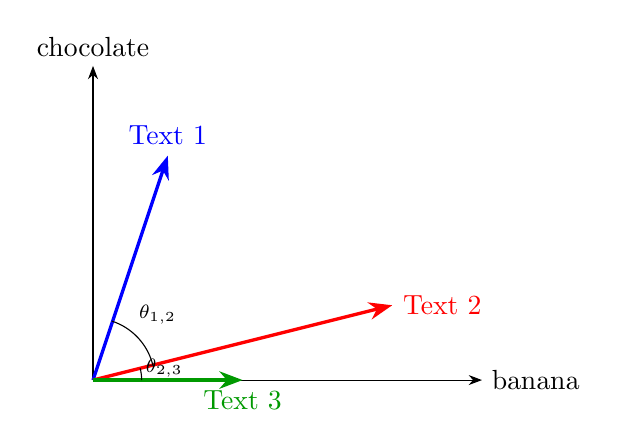
\begin{tikzpicture}[scale=.95,>=Stealth]
\draw[->] (0,0)--(5.2,0) node[right]{banana};
\draw[->] (0,0)--(0,4.2) node[above]{chocolate};
\draw[->,very thick,blue] (0,0)--(1,3) node[above]{Text 1};
\draw[->,very thick,red] (0,0)--(4,1) node[right]{Text 2};
\draw[->,very thick,green!60!black] (0,0)--(2,0) node[below]{Text 3};
\draw (.65,0) arc[start angle=0,end angle=14,radius=.65];
\node at (.95,.16) {\scriptsize$\theta_{2,3}$};
\draw (.8,.20) arc[start angle=14,end angle=72,radius=.83];
\node at (.86,.87) {\scriptsize$\theta_{1,2}$};
\end{tikzpicture}
\end{frame}

% 52
\begin{frame}{Vector Distances}
\[
d_E(x,y)=\sqrt{\sum_i(x_i-y_i)^2}
\qquad
d_M(x,y)=\sum_i|x_i-y_i|
\]
For Text 1 $(1,3)$ and Text 2 $(4,1)$:
\[
d_E(T1,T2)=\sqrt{(1-4)^2+(3-1)^2}=\sqrt{13}\approx3.61
\]
\[
d_M(T1,T2)=|1-4|+|3-1|=5
\]
\end{frame}

% 53
\begin{frame}{Euclidean vs. Manhattan Distance}
\centering
\begin{tikzpicture}[scale=.95,>=Stealth]
\draw[->] (0,0)--(5.2,0) node[right]{banana};
\draw[->] (0,0)--(0,4.2) node[above]{chocolate};
\fill[blue] (1,3) circle (2.4pt) node[above left]{Text 1 (1,3)};
\fill[red] (4,1) circle (2.4pt) node[below right]{Text 2 (4,1)};
\draw[red,dashed,thick] (1,3)--(4,1) node[midway,below]{$d_E$};
\draw[orange,dotted,thick] (1,3)--(4,3)--(4,1);
\node[orange] at (4.25,2) {$d_M$};
\end{tikzpicture}
\end{frame}

% 54
\begin{frame}{From Two Dimensions to Thousands}
\begin{itemize}
\item Real vocabularies are large
\item A document-term matrix can easily have tens of thousands of columns
\item Same logic as the two-dimensional example
\item Same math, but no longer visually intuitive
\end{itemize}
\end{frame}

\begin{frame}[plain]
  \centering
  \vfill
  {\usebeamercolor[fg]{structure}\LARGE\bfseries
   Feature engineering \& preprocessing \par}
  \vfill
\end{frame}


% Feature engineering: columns and values in the document-term matrix.
\begin{frame}{Feature Engineering}
\begin{itemize}
\item A \textbf{feature} is a property of a document recorded in the data matrix.
\end{itemize}
\vspace{.6em}
\[
X_{ij}=\text{value of feature }j\text{ for document }i
\]
\vspace{.6em}
\begin{itemize}
\item \textbf{Which columns?} Single words, phrases, or other properties of the text.
\item \textbf{What values?} Counts, 0/1 presence, or weights such as TF--IDF.
\end{itemize}
\vspace{1em}
These choices define what the matrix can capture.
\end{frame}

\begin{frame}{Which Columns Are in the Matrix?}
\textbf{Two documents}\\[.3em]
\quad D1: ``climate change matters''\qquad D2: ``climate policy matters''
\vspace{1em}
\small
\begin{tabular}{p{.27\textwidth}p{.63\textwidth}}
\toprule
\textbf{Choice} & \textbf{Possible columns}\\
\midrule
Unigrams & climate, change, policy, matters\\[.35em]
Add bigrams & climate\_change, change\_matters, climate\_policy, policy\_matters\\[.35em]
Require \texttt{min\_df=2} & climate, matters (each appears in both documents)\\
\bottomrule
\end{tabular}
\vspace{1em}
\normalsize
Adding phrases creates columns.
\end{frame}

\begin{frame}{What Goes in Each Cell?}
\textbf{Two documents}\\[.3em]
\quad D1: ``climate climate policy''\qquad D2: ``climate policy''
\vspace{1em}
\centering
\begin{tabular}{c|cc|cc}
& \multicolumn{2}{c|}{\textbf{Counts}} & \multicolumn{2}{c}{\textbf{Binary presence}}\\
& climate & policy & climate & policy\\
\midrule
D1 & 2 & 1 & 1 & 1\\
D2 & 1 & 1 & 1 & 1\\
\end{tabular}
\vspace{1.1em}
\begin{itemize}
\item Binary values discard repetition within a document.
\item TF--IDF rescales counts using how widely terms occur in the corpus.
\end{itemize}
\end{frame}

% 55
\begin{frame}{Text Preprocessing}
\begin{itemize}
\item Texts are highly dimensional
\item Preprocessing reduces dimensionality and standardizes features
\item But preprocessing is not neutral
\item It decides which distinctions are signal and which are noise
\end{itemize}
\end{frame}

% 56
\begin{frame}{Common Preprocessing Choices}
\begin{itemize}
\item Punctuation
\item Numbers
\item Lowercasing
\item Stemming / lemmatization
\item Stop-word removal
\item N-grams
\item Removal of words by frequency
\end{itemize}
\vspace{.4em}
{\tiny Based on common preprocessing decisions discussed in text-as-data workflows, including Denny \& Spirling (2018).}
\end{frame}

% 57
\begin{frame}{Punctuation / Numbers / Lowercasing}
\begin{itemize}
\item Often we remove punctuation and/or numbers
\item Often we lowercase all text
\item This reduces dimensionality
\item But it can remove meaningful distinctions
\end{itemize}
\vspace{.4em}
Is Trump the same as trump?\\
Is \term{Article 5} meaningful?\\
Does \term{!!!} matter in social media text?\\
Is \term{COVID-19} just noise?
\end{frame}

% 58
\begin{frame}{Lowercasing}
\begin{columns}[T]
\begin{column}{.48\textwidth}
\textbf{Can help}
\begin{itemize}
\item reduces vocabulary size
\item combines accidental variants
\item useful for many BoW tasks
\end{itemize}
\end{column}
\begin{column}{.48\textwidth}
\textbf{Can hurt}
\begin{itemize}
\item names and entities
\item acronyms
\item German nouns
\item stylistic emphasis
\end{itemize}
\end{column}
\end{columns}
\end{frame}

% 59
\begin{frame}{Stemming / Lemmatization}
\begin{itemize}
\item A stem is the part of the word responsible for lexical meaning
\item A stem is the invariable part of the word under inflection
\item "wait" is a stem of:
  \begin{itemize}\item waiting\item waits\item waited\end{itemize}
\item A \textbf{lemma} is the base or dictionary form
  \begin{itemize}\item "went", "gone" $\Rightarrow$ "go"\end{itemize}
\end{itemize}
\end{frame}

% 60
\begin{frame}{Stemming / Lemmatization: Why It Matters}
\begin{itemize}
\item Useful for dimension reduction
\item Often helps when measuring broad lexical content
\item But it can erase meaningful stylistic or grammatical distinctions
\end{itemize}
\vspace{.7em}
\begin{block}{Question}
When would you want to keep inflected forms separate?
\end{block}
\end{frame}

% 61
\begin{frame}{Stop Words}
\begin{itemize}
\item Words filtered out before analysis begins
\item Usually function words:
  \begin{itemize}\item the\item is\item that\item and\end{itemize}
\item Domain-specific words are also often excluded
  \begin{itemize}\item e.g., "climate" in a corpus about climate change\end{itemize}
\end{itemize}
\end{frame}

% 62
\begin{frame}{Stop Words Are Not Always Useless}
\begin{itemize}
\item Function words may be crucial for authorship attribution
\item Pronouns may matter for populism, identity, or blame attribution
\item Negation words matter: not, never, no
\item Modal verbs may matter: must, should, can
\end{itemize}
\end{frame}

% 63
\begin{frame}{N-grams}
\begin{itemize}
\item So far, we have mostly used unigrams: individual words
\item Texts can also be represented as sequences of $n$ words
\item Example: "I love ice-cream and bananas"
  \begin{itemize}
  \item unigrams: "I", "love", "ice-cream", "and", "bananas"
  \item bigrams: "I love", "love ice-cream", "ice-cream and", "and bananas"
  \end{itemize}
\end{itemize}
\end{frame}

% 64
\begin{frame}{Why N-grams?}
\centering
\begin{tabular}{ll}
\toprule
\textbf{Unigrams} & \textbf{N-gram meaning}\\ \midrule
climate, change & climate change\\
fake, news & fake news\\
not, good & not good\\
European, Union & European Union\\
social, media & social media\\
\bottomrule
\end{tabular}
\vspace{1em}
\begin{itemize}\item N-grams partly recover information lost by bag-of-words\end{itemize}
\end{frame}

% 65
\begin{frame}{Removal of Terms by Frequency}
\begin{itemize}
\item Further dimensionality reduction can be achieved by removing:
  \begin{itemize}
  \item very frequent terms
  \item very infrequent terms
  \end{itemize}
\item Very frequent terms may not discriminate between documents
\item Very infrequent terms may have low statistical power
\item But rare terms can still be substantively important
\end{itemize}
\end{frame}

% 66
\begin{frame}{Preprocessing Order Matters}
\centering
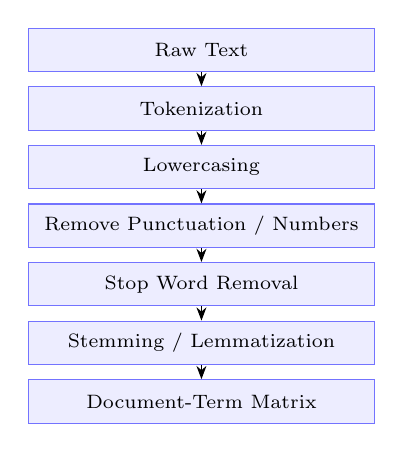
\begin{tikzpicture}[>=Stealth,box/.style={draw=blue!55,fill=blue!7,minimum width=4.4cm,minimum height=.55cm,align=center,font=\scriptsize},node distance=.18cm]
\node[box] (raw) {Raw Text};
\node[box,below=of raw] (tok) {Tokenization};
\node[box,below=of tok] (low) {Lowercasing};
\node[box,below=of low] (pun) {Remove Punctuation / Numbers};
\node[box,below=of pun] (stop) {Stop Word Removal};
\node[box,below=of stop] (stem) {Stemming / Lemmatization};
\node[box,below=of stem] (dtm) {Document-Term Matrix};
\draw[->] (raw)--(tok);\draw[->] (tok)--(low);\draw[->] (low)--(pun);
\draw[->] (pun)--(stop);\draw[->] (stop)--(stem);\draw[->] (stem)--(dtm);
\end{tikzpicture}
\end{frame}

% 67
\begin{frame}{Preprocessing Changes the Estimand}
\begin{itemize}
\item Suppose we remove punctuation, numbers, stop words, and word order
\item We are no longer measuring "language use" in general
\item We are measuring lexical content after discarding:
  \begin{itemize}
  \item style \quad syntax \quad discourse markers
  \item many forms of emphasis \quad some forms of negation
  \end{itemize}
\item This may be exactly what we want, but it should be a choice, not a default
\end{itemize}
\end{frame}

\begin{frame}[plain]
  \centering
  \vfill
  {\usebeamercolor[fg]{structure}\LARGE\bfseries
   Raw counts and TF-IDF \par}
  \vfill
\end{frame}


% 68
\begin{frame}{Beyond Raw Counts}
\begin{itemize}
\item A document-term matrix usually contains raw counts
\item But raw counts are not always ideal
\item Very frequent words dominate
\item Longer documents have larger counts
\item Some words are common everywhere and not very distinctive
\end{itemize}
\end{frame}

% 69
\begin{frame}{TF-IDF}
\begin{itemize}
\item We can do more than just count words
\item We can transform counts using weights
\item TF-IDF stands for:
  \begin{itemize}
  \item term frequency
  \item inverse document frequency
  \end{itemize}
\item Intuition: important terms are frequent in a document but rare across the corpus
\end{itemize}
\end{frame}

% 70
\begin{frame}{TF-IDF: Term Frequency -- Inverse Document Frequency}
\begin{itemize}
\item \textbf{TF:} how often a term appears in a document
\item \textbf{IDF:} downweight terms that appear in many documents
\end{itemize}
\[
\operatorname{TF\!-\!IDF}(t,d)=
\underbrace{\frac{\operatorname{count}(t,d)}
{\sum_{t'}\operatorname{count}(t',d)}}_{\mathrm{TF}}
\times
\underbrace{\log\frac{N}{\operatorname{df}(t)}}_{\mathrm{IDF}}
\]
\begin{itemize}
\item $N$ = total number of documents
\item $\operatorname{df}(t)$ = number of documents containing term $t$
\end{itemize}
\end{frame}

% 71: five Beamer overlays, matching five PDF pages
\begin{frame}{TF-IDF: What the hell?}
\begin{itemize}
\item It looks arbitrary because it partly is
\pause
\item Introduced by Karen Spärck Jones in 1972
\pause
\item Not derived from a deep theory of meaning
\pause
\item It is a useful heuristic: frequent in this document, rare elsewhere
\pause
\item Often works surprisingly well as a baseline
\end{itemize}
\end{frame}

% 72
\begin{frame}{What TF-IDF Is Useful For}
\begin{itemize}
\item Search and information retrieval
\item Finding characteristic words in documents
\item Document similarity
\item Clustering
\item Baseline features for supervised classification
\end{itemize}
\end{frame}

% 73
\begin{frame}{What TF-IDF Is Not}
\begin{itemize}
\item It is not a direct measure of how much a concept appears
\item It downweights common words even if they are theoretically important
\item It changes the interpretation of word counts
\item A high TF-IDF word is distinctive, not necessarily substantively important
\end{itemize}
\end{frame}

\begin{frame}[plain]
  \centering
  \vfill
  {\usebeamercolor[fg]{structure}\LARGE\bfseries
   Comparing documents and groups \par}
  \vfill
\end{frame}

% 74
\begin{frame}{Comparing Texts}
Once we represent texts as vectors, we can compare them.
\begin{itemize}
\item Which documents are most similar?
\item Which documents are outliers?
\item Which documents cluster together?
\item Which documents are closest to a query?
\end{itemize}
\end{frame}

% 75
\begin{frame}{Comparing Groups}
Sometimes we do not only compare documents.
\begin{itemize}
\item Which words are distinctive of one group?
\item Which words distinguish one corpus from another?
\item Which words are associated with one party, outlet, period, or actor?
\end{itemize}
Examples:
\begin{itemize}
\item tabloids vs. broadsheets
\item left parties vs. right parties
\item before vs. after an event
\item pro-government vs. opposition actors
\end{itemize}
\end{frame}

% 76
\begin{frame}{Odds}
\begin{itemize}
\item \textbf{Probability:} $p=\frac{\#\text{ successes}}{\#\text{ trials}}$
\item \textbf{Odds:} ratio of probability of success to probability of failure
\end{itemize}
\[
\mathrm{Odds}=\frac{p}{1-p}
\]
If $p=0.8$, then:
\[
\mathrm{Odds}=\frac{0.8}{0.2}=4
\]
4-to-1 in favor
\end{frame}

% 77
\begin{frame}{Log Odds}
\begin{itemize}
\item Log odds are the natural logarithm of odds
\item They map probabilities $(0,1)$ to the full real line $(-\infty,+\infty)$
\end{itemize}
\[
\operatorname{logit}(p)=\log\left(\frac{p}{1-p}\right)
\]
If $p=0.8$, then:
\[
\log\left(\frac{0.8}{0.2}\right)=\log(4)\approx1.39
\]
\end{frame}

% 78
\begin{frame}{Comparing Two Groups}
\begin{itemize}
\item Suppose we have two groups, for example John and Mary
\item Each group has its own probability of using a word
\item We compare their log odds
\end{itemize}
\[
\mathrm{Log\ Odds\ Ratio}=
\log\left(\frac{p_1}{1-p_1}\right)-
\log\left(\frac{p_2}{1-p_2}\right)
\]
\begin{itemize}
\item Positive value: word is more associated with group 1
\item Negative value: word is more associated with group 2
\end{itemize}
\end{frame}

% 79
\begin{frame}{Worked Example: "banana"}
\small
\begin{itemize}
\item John says "banana" in 7 out of 12 words: $p_1=7/12\approx0.58$
\item Mary says "banana" in 1 out of 16 words: $p_2=1/16=0.0625$
\end{itemize}
\[
\begin{aligned}
\mathrm{Log\ Odds\ Ratio}
&=\log\left(\frac{0.58}{0.42}\right)
-\log\left(\frac{0.0625}{0.9375}\right)\\
&=\log(1.38)-\log(0.0667)\\
&\approx0.32-(-2.71)\approx3.03
\end{aligned}
\]
Positive log-odds ratio $\Rightarrow$ "banana" is more associated with John.
\end{frame}

% 80
\begin{frame}{Why Use Log Odds?}
\begin{itemize}
\item Probabilities are bounded between 0 and 1
\item Odds ratios can be very skewed
\item Log odds:
  \begin{itemize}
  \item are symmetric around 0
  \item have direction and magnitude
  \item are related to logistic regression
  \item are useful for comparing word usage between groups
  \end{itemize}
\item In text analysis, log-odds approaches are often used to find distinctive words
\end{itemize}
\end{frame}

\begin{frame}[plain]
  \centering
  \vfill
  {\usebeamercolor[fg]{structure}\LARGE\bfseries
   Choosing a representation \par}
  \vfill
\end{frame}

% 81
\begin{frame}{Representation Choice Matrix}
\scriptsize
\centering
\begin{tabular}{p{.22\textwidth}p{.33\textwidth}p{.31\textwidth}}
\toprule
\textbf{Goal} & \textbf{Useful representation} & \textbf{Risk}\\ \midrule
Measure word prevalence & raw counts / proportions & common words dominate\\
Find distinctive terms & TF-IDF / log odds & distinctiveness $\neq$ importance\\
Compare documents & TF-IDF + cosine similarity & length and preprocessing matter\\
Capture phrases & n-grams & feature explosion\\
Reduce dimensionality & trimming / stemming & loss of meaning\\
Measure style & keep function words / punctuation & noisy features\\
\bottomrule
\end{tabular}
\end{frame}

% 82
\begin{frame}{Representation Choices Are Research Choices}
\begin{itemize}
\item If you remove stop words, you probably cannot study style well
\item If you remove numbers, you may lose dates, prices, laws, or percentages
\item If you use unigrams, you may miss fixed phrases
\item If you use TF-IDF, you are measuring distinctiveness, not raw prevalence
\item If you aggregate to documents, you may lose sentence-level meaning
\end{itemize}
\end{frame}

% 83
\begin{frame}{No Universal "Correct" Preprocessing}
\begin{block}{Bad question}
What is the correct preprocessing pipeline?
\end{block}
\vspace{1.5em}
\begin{block}{Better question}
What preprocessing pipeline is appropriate for this research question, corpus, and validation strategy?
\end{block}
\end{frame}

% 84
\begin{frame}{Beyond Bag-of-Words}
\begin{itemize}
\item Bag-of-words represents documents by explicit word counts.
\item This is simple, transparent, and often useful.
\item But it treats words as independent features.
\item It does not know that:
  \begin{itemize}
  \item "car" and "automobile" are similar
  \item "good" and "not good" are different
  \item the same word can mean different things in different contexts
  \end{itemize}
\item Later in the course, we will move from count-based representations to learned representations.
\end{itemize}
\end{frame}

% 85
\begin{frame}{Distributional Hypothesis}
\begin{itemize}
\item \textbf{Key idea:} words that occur in similar contexts tend to have similar meanings.
\item "You shall know a word by the company it keeps."
\item This motivates representing words by their contexts.
\item Instead of asking only how often a word appears, we ask:
  \begin{itemize}
  \item Which words appear near it?
  \item Which documents does it appear in?
  \item Which contexts is it associated with?
  \end{itemize}
\end{itemize}
\end{frame}

% 86
\begin{frame}{Preview: Word Embeddings}
\begin{itemize}
\item Word embeddings represent words as dense vectors.
\item Similar words should be close together in vector space.
\item Unlike bag-of-words, the dimensions are learned and not directly interpretable.
\item Embeddings are useful for:
  \begin{itemize}
  \item semantic similarity
  \item measuring concepts with word lists
  \item document representations
  \item transformers and LLMs
  \end{itemize}
\item We return to this in detail on Day 4.
\end{itemize}
\end{frame}

\begin{frame}[plain]
  \centering
  \vfill
  {\usebeamercolor[fg]{structure}\LARGE\bfseries
   Practical session \par}
  \vfill
\end{frame}

\begin{frame}{Practical Session: Guided Walkthrough}
\begin{itemize}
\item Work through notebook sections 1--8 together.
\item Start with a small toy corpus, then use State of the Union speeches.
\item Build word counts and TF--IDF representations.
\item Inspect distinctive words and document similarity.
\end{itemize}
\vspace{0.8em}
\textbf{Then:} Section 9 is your own short comparison.
\end{frame}

\begin{frame}{Your Turn: Change One Representation}
In notebook section 9, change only \texttt{task\_choice}. Use the same speeches.
\vspace{0.6em}
\begin{itemize}
\item \texttt{min\_df}: keep terms appearing in at least 5 speeches instead of 2.
\item \texttt{binary}: count whether a term appears in a speech (0/1), not repetitions.
\item \texttt{bigrams}: keep single words and add adjacent word pairs.
\end{itemize}
\vspace{0.5em}
Choose \textbf{one} option and rerun the student-task cell.
\end{frame}

\begin{frame}{Compare the Two Versions}
The cell prints a baseline and your changed representation.
\begin{itemize}
\item How many features does each version have?
\item Which terms were added or removed?
\item Did the top terms change? What do the totals mean in each version?
\item Which recent speech pairs changed most in cosine similarity?
\end{itemize}
\vspace{0.5em}
\textbf{Remember:} A small change in top terms can still hide a large change in the vocabulary or similarities.
\end{frame}

\begin{frame}{Discussion: What Did Your Choice Do?}
Write three sentences:
\begin{enumerate}
\item What changed between baseline and your version?
\item Why did this representation produce that change?
\item Which version better fits a research question you care about?
\end{enumerate}
\vspace{0.8em}
\textbf{Optional extension:} Compare speeches from 1950--79 with those from 1980 onward. This changes the groups being compared, rather than the representation.
\end{frame}

% 91
\begin{frame}{Key Takeaways}
\begin{itemize}
\item Text analysis begins with representation
\item A document-term matrix is simple but powerful
\item Bag-of-words is not stupid: it is a deliberate abstraction
\item Preprocessing is not cleaning: it is measurement design
\item TF-IDF and log odds help identify distinctive language
\item Different representations support different claims
\end{itemize}
\end{frame}

% 92
\begin{frame}{The Main Lesson}
\centering
\vspace{1em}
{\Large There is no raw text analysis.}
\vspace{2em}

{\Large There is always a representation.}
\vspace{2em}

A representation decides what counts as signal, what counts as noise, and what kind of claim the analysis can support.
\end{frame}

% 93
\begin{frame}{Tomorrow}
\begin{itemize}
\item Dictionaries and regular expressions
\item Human annotation and codebooks
\item Supervised machine learning
\item Evaluating classification models
\end{itemize}
\end{frame}

\end{document}
